\part{Introduzione alla CPU}

\chapter{Architettura di Von Neumann}
Il modello di von Neumann rappresenta in modo molto schematico le principali componenti hardware di un computer e le loro interconnessioni. Questa architettura è divisa in:
\begin{wrapfigure}{r}{0.4\textwidth}
        \begin{center}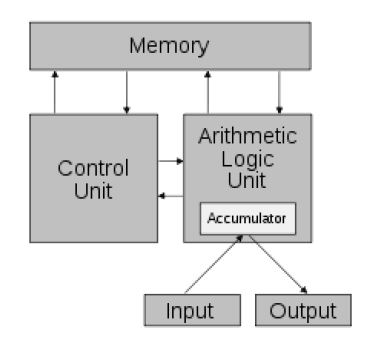
\includegraphics[width=6cm]{images/von_neumann.JPG}\end{center}
    \caption{Architettura di Von Neumann}
    \label{fig:von_neumann}
\end{wrapfigure}
\begin{itemize}
    \item \textbf{CPU} (Central Processing Unit o processore). E' formata da ALU (Unità Aritemtica Logica) che contiene tutti i circuiti per eseguire le operazioni aritmetico-logiche e la CU (o unità di controllo) per l’esecuzione dei programmi;
    \item \textbf{Memoria}. Nell’architettura dei calcolatori, si distinguono due tipi di memoria: la memoria centrale primaria, che lavora a diretto contatto con il processore e la memoria secondaria o di massa;
    \item \textbf{Periferiche di Input/Output}. Sono tutti quei dispositivi che non appartengono alla CPU o alla memoria (tastiera, schermo, stampante, scheda di rete ecc.);
    \item \textbf{Bus}. La CPU, la memoria e i dispositivi di Input/Output si scambiano i dati attraverso il Bus. Il Bus è l’insieme di linee su cui viaggiano i segnali elettrici formati da 0 e 1.
\end{itemize}


\chapter{Assembler MIPS}
\section{Architetture CISC e RISC}\label{architettureCISCeRISC}
Possiamo distinguere due macro categorie di architetture, che si basano su due filosofie diverse:
\begin{itemize}
    \item \textbf{CISC} (Complex Instruction Set Computer), sono le prime a nascere ma sono allo stesso tempo le più complesse (contengono più microistruzioni) ed inoltre si basano sull'accesso in memoria (quindi anche gli indirizzamenti saranno adattati a questa filosofia).
    \item \textbf{RISC} (Reduced Instruction Set Computer), nascono successivamente. Le istruzioni sono poco complesse ed inoltre si basano sui registri. La filosofia è quella di far parlare più instruzioni in meno tempo possibile. Non è realmente importante la velocità di esecuzione delle istruzioni stesse.
\end{itemize}

\section{MIPS}

Il \textbf{MIPS} (Microprocessor without Interlocked Pipelined Stages) è di tipo RISC. Nel MIPS gli operandi devono essere contenuti nei registri per potere eseguire delle operazioni.

Alla memoria si accede solamente attraverso le istruzioni di trasferimento dati. Il MIPS utilizza l'indirizzamento al byte, perciò due parole consecutive hanno indirizzi in memoria a una distanza di 4. La memoria consente di memorizzare strutture dati, vettori, o il contenuto dei registri.\\

Tramite il linguaggio assembler MIPS possiamo svolgere diverse operazioni:
\begin{figure}
    \centering
    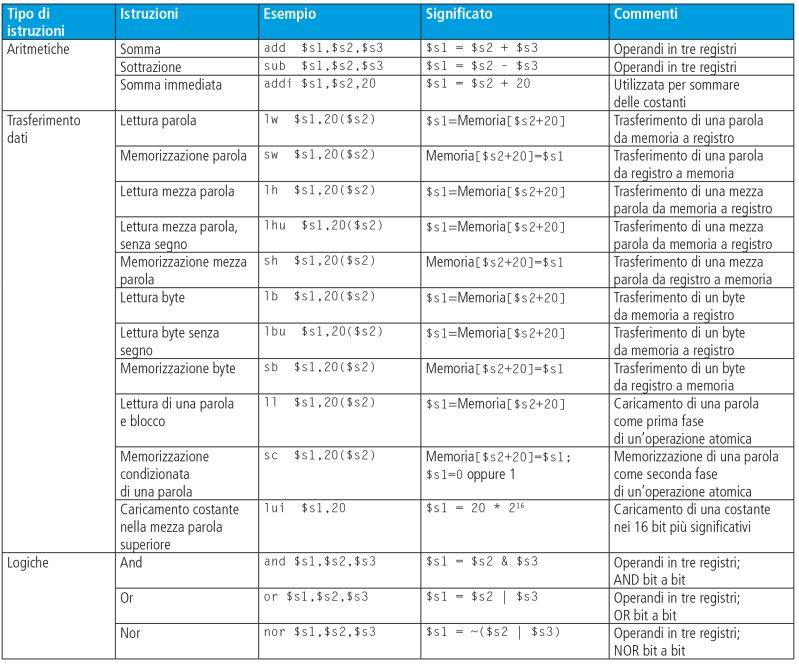
\includegraphics[width=15cm]{images/operazioni_MIPS.JPG}
    \label{fig:operazioni_mips}
\end{figure}
\begin{figure}
    \centering
    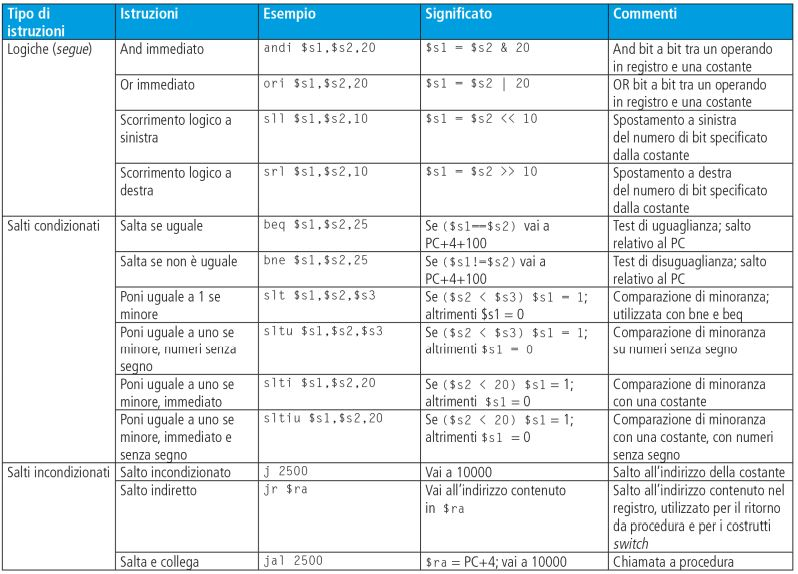
\includegraphics[width=15cm]{images/operazioni_MIPS_2.JPG}
    \label{fig:operazioni_mips_2}
\end{figure}

\section{Rappresentazione dell'istruzione}
Le istruzioni della CPU sono formate tutte da 32 bit con formato molto simile. Distinguiamo i tipi di rappresentazione in tre formati in base al numero di registri utilizzati e alle operazioni svolte:
\begin{itemize}
    \item \textbf{R-type} istruzioni senza accesso alla memoria e con istruzioni aritmetico$\backslash$logiche;
    \item \textbf{I-type} istruzioni di trasferimento immediato;
    \item \textbf{J-type} istruzioni di salto.
\end{itemize}


\subsection*{R-type}
Con la rappresentazione R-type occupiamo 6 bit per l'opcode, che rappresenta la classe di operazioni. 5 bit per l'rs, ovvero il primo registro dell'operazione e la stessa cosa avviene con rt, il secondo registro dell'operazione e rd il registro destinazione. 5 bit anche per lo shamt o shift amount, indice il valore dello shift. Infine 6 bit per il funct o funcion code, rappresenta il codice dell'operazione da svolgere.

\begin{table}[H]
    \centering
    \begin{tabular}{|p{1.5cm}|p{1.5cm}|p{1.5cm}|p{1.5cm}|p{1.5cm}|p{1.5cm}|}
         \hline \large{op} & \large{rs} & \large{rt} & \large{rd} & \large{shamt} & \large{funct}\\\hline
    \end{tabular}
\end{table}

Ad esempio effettuando \textit{add \$t0, \$s1, \$s2} otteniamo:

\begin{table}[H]
    \centering
    \begin{tabular}{|p{1.5cm}|p{1.5cm}|p{1.5cm}|p{1.5cm}|p{1.5cm}|p{1.5cm}|}
         \hline \large{000000} & \large{10001} & \large{10010} & \large{01000} & \large{00000} & \large{100000}\\\hline
    \end{tabular}
\end{table}

Notiamo che i registri da \$s0 a \$s7 corrispondono agli indirizzi 16-23 mentre i registri da \$t0 a \$t7 corrispondono agli indirizzi 8-15.

\subsection*{I-type}
Con la rappresentazione I-type vengono rimpiazzati i 16 bit di rd, shamt e funct con constant or address che conterrà un totale di 16 bit:

\begin{table}[H]
    \centering
    \begin{tabular}{|p{1.5cm}|p{1.5cm}|p{1.5cm}|p{4.5cm}|}
         \hline \large{op} & \large{rs} & \large{rt} & \large{constant or address}\\\hline
    \end{tabular}
\end{table}


\subsection*{J-type}
Le unice istruzioni di salto sono le \verb|j| e \verb|jal|. Con la rappresentazione J-type utilizziamo solamente l'op e l'indirizzo di destinazione:
\begin{table}[H]
    \centering
    \begin{tabular}{|p{1.5cm}|p{7.5cm}|}
         \hline \large{op} & \large{\hspace{3cm} address}\\\hline
    \end{tabular}
\end{table}

\section{Tipi di indirizzamento alla memoria}
\subsection*{Organizzazione della memoria}
Dobbiamo immaginare la memoria come una pila di elementi indirizzati. Gli indirizzi di memoria vengono contati a multipli di quattro. Partendo da queste precisazioni seguiamo lo schema proposto in Figura \ref{fig:organ_mem}, dove il PC (Program Counter) è un registro contatore la cui funzione è quella di conservare l'indirizzo di memoria della prossima istruzione da eseguire. Il GP (Global Pointer) è un registro usato per accedere tramite un offset
alla sezione data. Lo SP (Stack Pointer) è un registro che contiene l’indirizzo di inizio dello stack.

\begin{figure}[H]
    \centering
    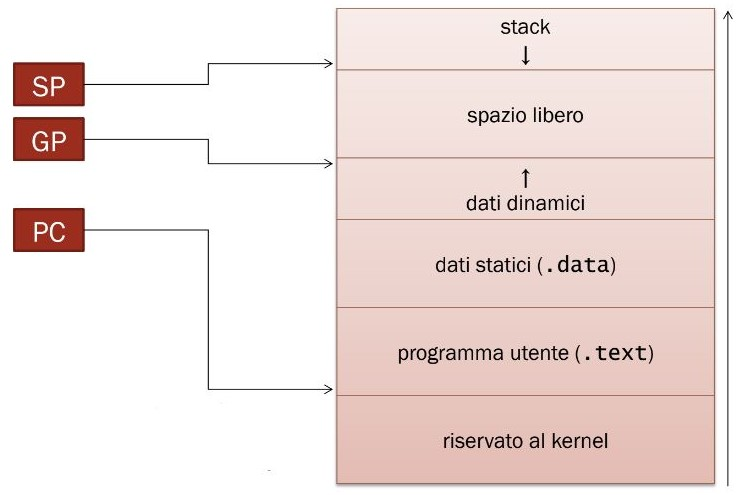
\includegraphics[width = 10cm]{images/organizzazione_memoria.JPG}
    \caption{Organizzazione della memoria}
    \label{fig:organ_mem}
\end{figure}

\subsection*{Cosa sa fare la CPU?}
Con l'IAS Machine abbiamo visto tutte le fasi di esecuzione di un'istruzione. Le tipologie di istruzioni che la CPU può svolgere sono:
\begin{itemize}
    \item \textbf{LOAD$\backslash$ STORE}. Trasferiscono dati da/verso la memoria. Es: \verb|lw|, \verb|lh|, \verb|lb|, \verb|sw|, \verb|sh|, \verb|sb|, \verb|lwc1|, \verb|swc1|.
    \item \textbf{Logico$\backslash$ Aritmetiche}. Svolgono i calcoli aritmetici e logici Es: \verb|add|, \verb|sub|, \verb|mul|, \verb|div|, \verb|sll|, \verb|srl|, \verb|sra|.
    \item \textbf{Salti condizionati e incondizionati}. Controllano il flusso logico di esecuzione. Es: \verb|j|, \verb|jal|, \verb|brqz|, \verb|blt|, \verb|ble|.
    \item \textbf{Gestione delle eccezioni/interrupt}. Salvataggio dello stato e suo ripristino. Es: \verb|eret|.
    \item \textbf{Istruzioni di trasferimento dati}.
\end{itemize}

\subsection*{Codifica delle istruzioni}
La codifica della istruzione indica quale operazione deve essere eseguita, tramite l'\verb|opcode|, e successivamente inserire il risultato di tale operazione tramite l'address o altri registri.

Esistono principalmente due tipi di indirizzamento. Il modo diretto guida direttamente alla cella di memoria. Il modo indiretto, invece, fa uso di un altro indirizzo che contiene un puntatore alla zona di memoria dove verrà inserito il risultato. Esistono anche altre due varianti di questi processi con i registri, dove nel primo caso il risultato viene direttamente inserito nel registro, mentre nel secondo il registro contiene l'indirizzo di memoria dell'address.

\begin{figure}[H]
    \centering
    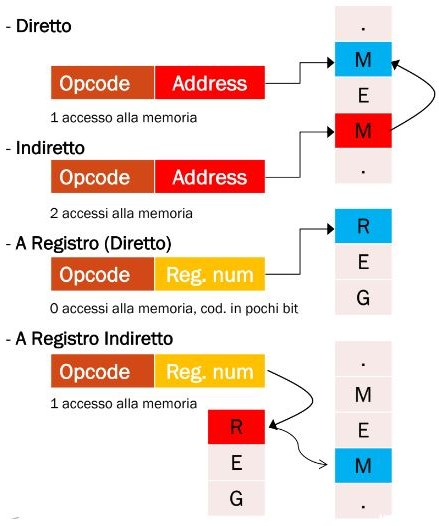
\includegraphics[width=6cm]{images/indirizzamenti_diretto_indiretto.JPG}
    \caption{Indirizzamenti diretti e indiretti}
    \label{fig:indirizz_diretti_indiretti}
\end{figure}

Esiste anche un modo più intelligente utilizzando lo spiazzamento.

\begin{wrapfigure}{r}{6cm}
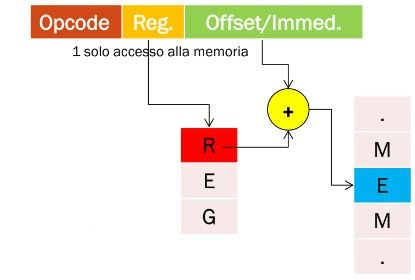
\includegraphics[width=6cm]{images/indirizzo_spiazzamento.JPG}
\end{wrapfigure} 

Questo metodo è più efficiente in quanto con quelli precedenti siamo obbligati a sommare e sottrarre indirizzi di memoria. Con questo tipo di indirizzamento tutto ciò non avviene perchè utilizziamo un registro dove viene inserito il valore interessato, che verrà calcolato successivamente. R rappresenta infatti il registro dove si trova l'accesso alla memoria mentre l'offset ci indica di quanto dobbiamo spostarci. Con un esempio sarà tutto più chiaro.
\begin{example*}
    Mi trovo ad indirizzo 0, $0xAAAB1234$, e voglio arrivare alla terza riga della pila, ovvero 8 (dato che gli indirizzi vengono contati di 4 in 4).
    
    Con i metodi visiti precedentemente doveri fare:
    \begin{equation*}
        0xAAAB1234+8=0xAAAB123C
    \end{equation*} e per tornare all'inizio dovrei sottrarre di nuovo 8.
    Mentre con lo spiazzamento effettuo:
    \begin{equation*}
        0xAAAB1234+\$s0x4
    \end{equation*}e in $\$s0$ inserisco il valore 2. Così ottengo $2x4=8$.
\end{example*}

\subsection*{MIPS 2000}
L’architettura MIPS 2000 è formata da 3 CPU:
\begin{itemize}
    \item Una prima CPU formata da 32 registri da 32 bit. Viene utilizzata per la moltiplicazioni e divisioni.
    \item Il coprocessore 0 che si occupa della memorizzazione e della cattura delle eccezioni.
    \item Il coporcessore 1 che viene utilizzato per i calcoli in virgola mobile.
\end{itemize}

\begin{figure}[H]
    \centering
    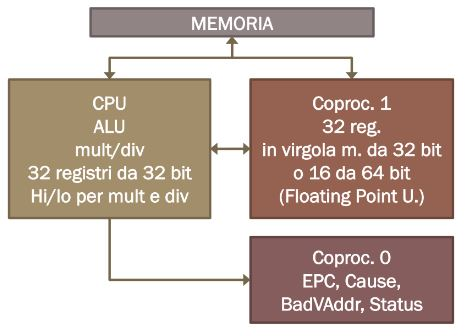
\includegraphics[width=8cm]{images/mips_2000.JPG}
    \caption{MIPS 2000}
    \label{fig:mips_2000}
\end{figure}

I 32 registri della CPU sono divisi come segue:
\begin{itemize}
    \item[] \verb|$zero| è un registro immutabile che contiene la costante zero;
    \item[] \verb|$at| usato dalle pseudoistruzioni;
    \item[] \verb|$v0,$v1| dove v sta per value. Tendenzialmente vengono inseriti i risultati delle funzioni;
    \item[] \verb|$a0..$a3| vengono utilizzati per contenere gli argomenti delle funzioni;
    \item[] \verb|$t0..$t7| sono registri temporanei salvati dal chiamante;
    \item[] \verb|$s0..$s7| sono temporanei salvati dal chiamato;
    \item[] \verb|$t8,$t9| altri registri temporanei salvati dal chiamante;
    \item[] \verb|$k0,$k1| kernel per eccezioni;
    \item[] \verb|$gp| global pointer (memoria dinamica);
    \item[] \verb|$sp| stack pointer (stack delle funzioni);
    \item[] \verb|$fp| frame pointer (funzioni);
    \item[] \verb|$ra| return address.
\end{itemize}


